% ------------------------------------------------------------------------
% -*-TeX-*- -*-Hard-*- Smart Wrapping
% ------------------------------------------------------------------------
\def\baselinestretch{1}

\chapter{Literature Review and Related Work}

\def\baselinestretch{1.66}


%%% ----------------------------------------------------------------------

% intro text here

\smallskip

%%% ----------------------------------------------------------------------
\goodbreak
\section{The Counting Problem}
A prevalent theme in the field of Computer Science is that of performing tasks traditional to humans, through the use of a computer. Counting is a trivial cognitive task for humans. In fact, it comes so naturally that studies have shown that children below the age of 3 demonstrate an understanding of numerosity without any knowledge of number or counting systems (\cite{REF1}). For a computer, the task of estimating the number of objects (of some kind) in an image is slightly more complicated and comes up in many real world applications such as counting cells in microscopic images and monitoring crowds in surveillance systems.\\ \\
%
The most established ways of counting objects in images involve the use of image processing or computer vision techniques in conjunction with machine learning methods. While there are are many different approaches which employ different techniques to achieve these goals, they all share (to some extent) the same general outline. The image is first transformed to greyscale. The greyscale image is thresholded to yield a binary image. The binary image is segmented and the features to be used for counting are extracted and passed into the model. Figure 1 shows a generalized flowchart for the activities involved in counting objects in images with the stages described as follows:\\
% _FIG_ Flowchart process image here
\begin{figure}[ht!]
\centering
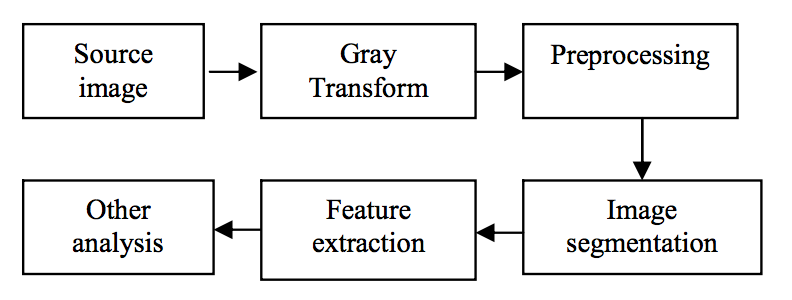
\includegraphics[scale=0.5]{Images/general_pipeline}
\caption{Generalized pipeline for approaching the counting problem}
\label{fig:columnfigure}
\end{figure}

\begin{description}
\item[(i)] \textbf{Gray Transform:} The image is first transformed to greyscale. This is because counting usually depends on morphological (ie. shape), spatial and textural features that have no use for colour. The exclusion of colour simplifies subsequent calculations and makes the whole process more computationally efficient. Also, a lot of the techniques used in processes further down the pipeline are designed to work on simple two-dimensional matrices and would be very difficult, if not impossible, to extend to colour images. There are various ways to achieve this conversion. One way is to simply average the RGB pixel values to give the greyscale pixel value (\cite{REF2}). A more accurate method of conversion is the use of a luminance-preserving mapping. This method gives the greyscal pixel value, given as the \textit{luminosity} of the pixel, to be calculated as a weighted sum of the RGB pixel values (\cite{REF3}).
\begin{equation}
Y = 0.2126R + 0.7152G + 0.0722B
\label{eqn:luminosity}
\end{equation}
Applying the formulae described above to each pixel in a colour image will result in a grayscale vesion of the image.\\ 

\item[(iii)] \textbf{Preprocessing:} The presence of noise in the image will affect the counting accuracy. Because of this, certain transformations must be carried out on the image before going further. Also, depending on the objects to be counted in an image, some processes can be performed on the image in order to highlight or de-emphasize appropriate elements of the image to make detection and counting easier and more reliable. Image smoothing and sharpening are usually used to achieve this. Image smoothing can be carried out by applying a \textit{Gaussian filter} (\cite{REF4}) or a \textit{median filter} (\cite{REF5}). However, in the process of removing noise from the image, image smoothing might also blur some of the edges in the image. Blurred edges are not conducive to segmentation, analysis and other potential follow-up processes. Hence, image sharpening is performed on the image in order to emphasize the edges in the image. Image sharpening can be carried out by applying a \textit{high-pass filter} (\cite{REF6}).\\

\item[(iii)] \textbf{Binary Image Segmentation:} Image segmentation is typically used to locate objects and boundaries (lines, curves, etc.) in images. More precisely, image segmentation is the process of assigning a label to every pixel in an image such that pixels with the same label share certain characteristics (\cite{REF7}). With binary image segmentation, which is what is usually used in object detection and counting, there is only one label - ``edge''. Pixels that form part of an edge are assigned a value of $1$ and any other pixel is assigned a value of $0$. Given this, image segmentation in this sense can be performed by applying an edge detection algorithm to the image. A popular edge detection algorithm used for image segmentation is the \textit{Canny edge detection} algorithm (\cite{REF8}). In simple terms, the Canny edge detection algorithm finds edges where the grayscale intensity of the image changes. These areas and changes can be approximated by calculating the gradient $G$ in the image in the $x$ and $y$ directions.\\
\begin{align*}
|G| = \sqrt{G_x^2 + G_y^2}\\
|G| = |G_x| + |G_y|\\
\theta = arctan(\frac{|G_x|}{|G_y|}) \tag{2}
\end{align*}

\item[(iv)] \textbf{Feature Extraction:} Feature extraction plays a very important role in the area of image processing with regards to machine learning. Feature extraction is a type of dimensionality reduction that efficiently represents interesting parts of an image as a compact feature vector (\cite{REF9}). These extracted vectors can then be used as inputs and elements of machine learning algorithms and techniques. The approach of using the extracted feature vectors instead of the entire image proves advantageous when image sizes are large. Using a reduced representation of the image makes it possible to perform many common and important tasks quickly. Common feature extraction techniques include Histogram of Oriented Gradients (HOG) (\cite{REF10}), Speeded Up Robust Features (SURF) (\cite{REF11}), color histograms (\cite{REF12}) and Scale-InvariantFeature Transform (SIFT) (\cite{REF13}).\\

\item[(v)] \textbf{Analysis:} In this stage, the extracted feature vector representation of the image has statistical models or machine learning algorithms applied to it in order to recognize, detect or count objects within the given image. The objective of the analysis stage is to learn some useful information from the image, and most times, all of the preceding stages are carried out solely in preparation for this stage.
\end{description}

% Talk about general process. Include diagram of stages. Explain stages

\bigskip

%%% ----------------------------------------------------------------------
\goodbreak

\section{Existing Approaches to Counting}
A lot of research has been carried out on counting objects in images. However, the objects being considered for counting differ from project to project. Because of this, there are a lot of different ideas and approaches to solving this problem. While they all seem to employ machine learning, some of the ideas take an unsupervised learning approach while others take a supervised learning approach. Supervised learning involves training a model with labeled instances of the subjects being investigated. Examples of these methods are machine learning classifiers. In unsupervised learning, the system is not introduced to any labeled training instances but learns on the job. An example of this is \textit{clustering}.\\ \\
%
A few approaches to solving the counting problem employ unsupervised learning by clustering or grouping similar aspects of the image. (\cite{REF14}) propose a method for grouping based on self-similarities and (\cite{REF15}) propose a method for grouping based on motion similarities. However, the counting accuracy of such fully unsupervised methods is limited, and therefore others considered approaches based on supervised learning. These approaches fall into the following categories:

\subsection{Counting by Detection}
These approaches solve the problem by first detecting the objects in question and then counting them. Object detection is carried out by the use of a visual object detector that localizes individual instances of the object in the image. Given the localizations of the objects' instances, counting becomes trivial. However, visual object detection is far from being solved and is even more tricky when overlapping instances are involved. Several methods assume that objects are uniform and disconnected from each other by the distinct background color. Following this assumption, it is possible to localize individual instances via the Monte-Carlo process (\cite{REF16}) or morphological analysis (\cite{REF17}). These methods yield reliable results when the assumption is met but are not so applicable in challenging real life situations. 

\subsection{Counting by Regression}
These approaches sidestep the hard detection problem altogether and instead, attempt to form a direct mapping from some features or groups of features of the image to the number of objects contained within it. This is a standard regression problem that can be addressed by many different machine learning tools such as neural networks. This approach however has to discard any available information about the location of the objects, using only its 1-dimensional statistics (total number) for learning. As a result, a large number of training images with the supplied counts needs to be provided during training (\cite{REF18}).


\bigskip

%%% ----------------------------------------------------------------------
\goodbreak
%%% ----------------------------------------------------------------------
\section{Texture Analysis for Feature Extraction}
Image texture analysis is a process which applies certain techniques to extract texture parameters from an image in order to quantify or qualify its perceived texture. Image texture gives us information about the spatial arrangement of color or intensities in an image or selected region of an image (\cite{REF21}). Generally speaking, textures are complex visual patterns that have characteristics such as brightness, colour and contrast. Because of this, texture is easily perceived by humans and is believed to be a rich source of visual information. Thus, texture is can be used as a metric for similarity between images.\\ \\
%
The proposed approach makes use of \textbf{\textit{Gray Level Co-occurrence Matrix (GLCM)}} texture analysis. A co-occurrence matrix can be defined as the distribution of co-occurring values at a given offset. It reflects the luminance distribution (as well as position distribution) between the same pixels or pixels with similar luminance values. The Gray Level Co-occurrence Matrix (GLCM) is formed from a gray-scale image and calculates how often a pixel with gray-scale intensity $i$ occurs (horizontally, vertically or diagonally) adjacent to pixels with gray-scale intensity $j$. Simply put, a GLCM characterizes an image by calculating how often pairs of pixels with specific values (and in a specified spatial relationship) occur in an image, where the spatial relationship could be horizontally adjacent, vertically adjacent or diagonally adjacent. The spatial relationship between pixels can be denoted using direction $\theta$ and distance $d$. For example, using this notation, the spatial relationship between two pixels $i$ and $j$ that are 3 pixels apart diagonally could be denoted as $(d,\theta) = (3,45^\circ)$.\\ \\
%%%%%%%%%%%%%%%%%%%%%%%%%%%%%%%%%%%%%%%%
%%%%%%%%%%%%%%%%%%%%%%%%%%%%%%%%%%%%%%%%
%%%%%%%%%%%%%%%%%%%%%%%%%%%%%%%%%%%%%%%%
%%%%%%% _FIG_ d,theta IMAGE HERE %%%%%%%%%%%%%
%%%%%%%%%%%%%%%%%%%%%%%%%%%%%%%%%%%%%%%%
%%%%%%%%%%%%%%%%%%%%%%%%%%%%%%%%%%%%%%%%
%%%%%%%%%%%%%%%%%%%%%%%%%%%%%%%%%%%%%%%%

\begin{figure}[ht!]
\centering
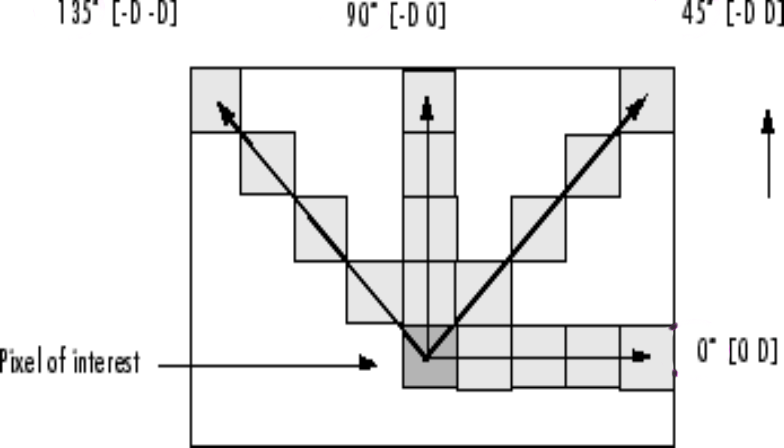
\includegraphics[scale=0.55]{Images/glcm_direction}
\caption{Illustration of GLCM spatial analysis (\cite{REF24})}
\label{fig:columnfigure}
\end{figure}

Below are the textural descriptors that can be derived from a GLCM $p$ with size $M$ by $N$:
\begin{itemize}
\item \textit{Energy}\\
\begin{align*}
ASM = \sum_{i=1}^{M}\sum_{j=1}^{N} p(i,j|d,\theta)^2
\end{align*}
is computed as the sum of squared elements in the GLCM. It is also known as \textit{uniformity}, \textit{uniformity of energy}, and \textit{angular second moment} and it represents texture coarseness.\\

\item \textit{Contrast}\\
\begin{align*}
CON = \sum_{i=1}^{M}\sum_{j=1}^{N} |i-j|^2p(i,j|d,\theta)^2
\end{align*}
returns a measure of the intensity contrast between a pixel and its neighbor over the whole image. It is also known as \textit{variance} and \textit{inertia}.

\item \textit{Homogeneity}\\
\begin{align*}
HOM = \sum_{i=1}^{M}\sum_{j=1}^{N} \frac{p(i,j|d,\theta)}{1 + |i - j|}
\end{align*}
represents the uniformity of the image and measures the change of local image texture.

\item \textit{Correlation}\\
\begin{align*}
CORR = \sum_{i=1}^{M}\sum_{j=1}^{N} \frac{(i -\mu_i)(j - \mu_j)p(i,j|d,\theta)}{\sigma_i\sigma_j}
\end{align*}
Returns a measure of how correlated a pixel is to its neighbour over the whole image.\\

\end{itemize}

\bigskip

%%% ----------------------------------------------------------------------
\goodbreak

\section{Learning and Modeling}
In order to solve the counting problem, some way of actually determining the number of objects present in a preprocessed representation of an image has to be established. This is usually done by building a model to be used to perform this determination using machine learning techniques. As explained above, supervised learning models yield better results and perform better in practice. A supervised learning model is built from previously encountered and labeled instances and is then applied to subsequently encountered instances.\\ \\
%
One possible tool for building such models is the \textit{support vector machine} (SVM). The Support vector machine is a machine learning tool that is usually used for classification tasks but can be extended to regression tasks as well. An SVM model is a representation of the training examples as points in space, mapped so that the examples of the separate classes are separated by a hyperplane (or set of hyperplanes in high dimension problems) while maximizing the distance from the hyperplanes to the nearest training point. Given a set $D$ of $n$ training points, 
\begin{equation}
D = \{(x_1, x_2)  \ldots  (x_n, y_n)\}
\end{equation}
with a hyperplane described by the equation
\begin{equation}
\langle w,x \rangle + b = 0
\end{equation}
To minimize the margin of the hyperplane, the idea is to solve the optimization problem
\begin{equation}
\text{minimize }||w||\text{ such that }y_i(\langle w,x \rangle - b) \ge 1, i = 1  \ldots  n 
\end{equation}\\
%
For non-linearly separable scenarios, a loss function may be applied to the SVM. Usually the hinge-loss function is used for this. SVMs can be extended to regression problems by the introduction of an alternative loss function (\cite{REF19}). The alternative loss function must be modified to include a distance measure. Some possible loss functions are the quadratic function, laplacian function and Huber function.\\ \\
%
Another machine learning tool that can be used for modeling is the \textit{artificial neural network}. Artificial neural networks are a family of machine learning models inspired by the way that biological nervous systems, such as the brain, process information. A neuron is a cell that has several inputs that can be activated by some outside process. Depending on the amount of activation, the neuron produces its own activity and sends this along its outputs (\cite{REF20}). In addition, specific input or output paths may be ``strengthened'' or weighted higher than other paths. The artificial neural network equivalent of a neuron is a \textit{\textbf{node}}. A node receives a set of (weighted) inputs, applies its activation function $\phi$ to their sum, and passes the result of the activation function to nodes further down the network. The activation function can thus be represented as such
\begin{equation}
\phi = \sum_{i=1}^{n} w_i.a_i
\end{equation}
Many such nodes are chained together to form a network, passing the outputs of their activation functions along. The network is trained with labeled data by feeding inputs into the network and fine-tuning the weights until the network always yields the expected class label as its output. This is not very different from regression in that parameters are being tuned to create a function that yields certain values. Hence, artificial neural networks can easily be adapted to solve regression problems.
% Maybe bias-variance as shown in lecture notes

\bigskip

%%% ----------------------------------------------------------------------

